\documentclass{standalone}
\usepackage{tikz}
\usetikzlibrary{patterns, positioning}
\usepackage[sfdefault]{ClearSans} %% option 'sfdefault' activates Clear Sans as the default text font
\usepackage[T1]{fontenc}

\begin{document}
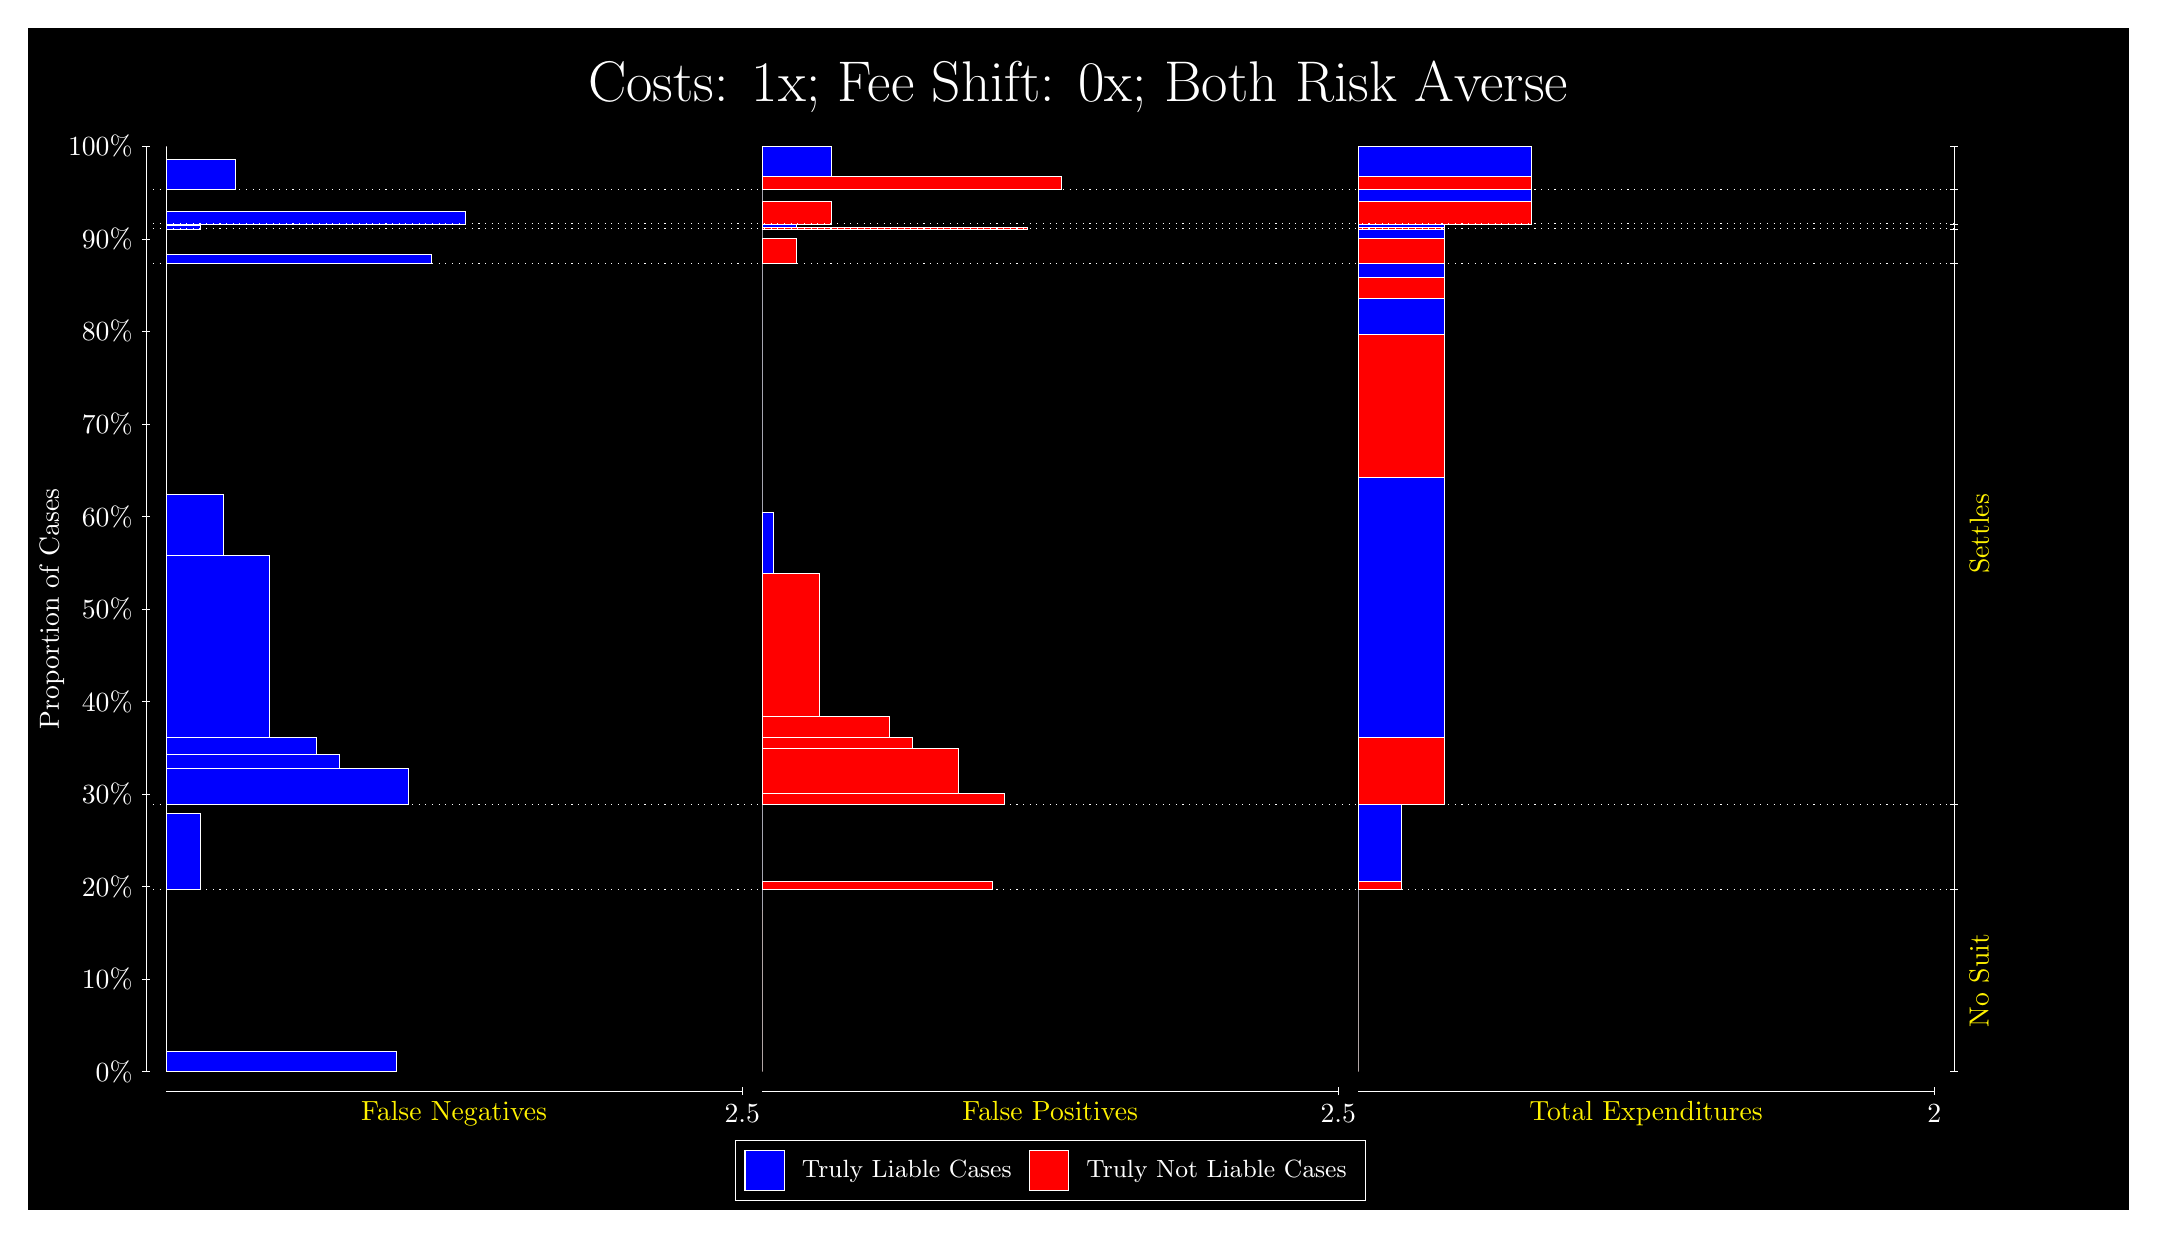
\begin{tikzpicture}
\draw[fill=black] (0,0) rectangle (26.667,15);
\draw[text=white] (0,13.5) rectangle (26.667,15) node[midway] {\huge Costs: 1x; Fee Shift: 0x; Both Risk Averse};
\draw[white, very thin] (1.5,1.75) -- (1.5,13.5);
\node[rotate=90, text=white, anchor=center] at (0.3, 7.625) {Proportion of Cases};
\draw[white, very thin] (1.45,1.75) -- (1.55,1.75);
\node[text=white, anchor=east] at (1.45, 1.75) {0\%};
\draw[white, very thin] (1.45,2.925) -- (1.55,2.925);
\node[text=white, anchor=east] at (1.45, 2.925) {10\%};
\draw[white, very thin] (1.45,4.1) -- (1.55,4.1);
\node[text=white, anchor=east] at (1.45, 4.1) {20\%};
\draw[white, very thin] (1.45,5.275) -- (1.55,5.275);
\node[text=white, anchor=east] at (1.45, 5.275) {30\%};
\draw[white, very thin] (1.45,6.45) -- (1.55,6.45);
\node[text=white, anchor=east] at (1.45, 6.45) {40\%};
\draw[white, very thin] (1.45,7.625) -- (1.55,7.625);
\node[text=white, anchor=east] at (1.45, 7.625) {50\%};
\draw[white, very thin] (1.45,8.8) -- (1.55,8.8);
\node[text=white, anchor=east] at (1.45, 8.8) {60\%};
\draw[white, very thin] (1.45,9.975) -- (1.55,9.975);
\node[text=white, anchor=east] at (1.45, 9.975) {70\%};
\draw[white, very thin] (1.45,11.15) -- (1.55,11.15);
\node[text=white, anchor=east] at (1.45, 11.15) {80\%};
\draw[white, very thin] (1.45,12.325) -- (1.55,12.325);
\node[text=white, anchor=east] at (1.45, 12.325) {90\%};
\draw[white, very thin] (1.45,13.5) -- (1.55,13.5);
\node[text=white, anchor=east] at (1.45, 13.5) {100\%};

\draw[white, very thin] (24.457,1.75) -- (24.457,13.5);
\draw[white, very thin] (24.407,1.75) -- (24.507,1.75);
\node[anchor=west] at (24.407, 1.75) {};
\draw[white, very thin] (24.407,4.06) -- (24.507,4.06);
\node[anchor=west] at (24.407, 4.06) {};
\draw[white, very thin] (24.407,5.1409) -- (24.507,5.1409);
\node[anchor=west] at (24.407, 5.1409) {};
\draw[white, very thin] (24.407,12.014) -- (24.507,12.014);
\node[anchor=west] at (24.407, 12.014) {};
\draw[white, very thin] (24.407,12.452) -- (24.507,12.452);
\node[anchor=west] at (24.407, 12.452) {};
\draw[white, very thin] (24.407,12.516) -- (24.507,12.516);
\node[anchor=west] at (24.407, 12.516) {};
\draw[white, very thin] (24.407,12.955) -- (24.507,12.955);
\node[anchor=west] at (24.407, 12.955) {};
\draw[white, very thin] (24.407,13.5) -- (24.507,13.5);
\node[anchor=west] at (24.407, 13.5) {};

\draw[white, very thin, fill=blue] (1.75,1.75) rectangle (4.6775,2.0085);
\draw[white, very thin, fill=red] (1.75,2.0085) rectangle (1.75,4.06);
\draw[white, very thin, fill=blue] (1.75,4.06) rectangle (2.1891,5.0312);
\draw[white, very thin, fill=red] (1.75,5.0312) rectangle (1.75,5.1409);
\draw[white, very thin, fill=blue] (1.75,5.1409) rectangle (4.8239,5.6047);
\draw[white, very thin, fill=blue] (1.75,5.6047) rectangle (3.9457,5.7826);
\draw[white, very thin, fill=blue] (1.75,5.7826) rectangle (3.6529,5.9902);
\draw[white, very thin, fill=blue] (1.75,5.9902) rectangle (3.0674,8.301);
\draw[white, very thin, fill=blue] (1.75,8.301) rectangle (2.4819,9.0825);
\draw[white, very thin, fill=red] (1.75,9.0825) rectangle (1.75,12.014);
\draw[white, very thin, fill=blue] (1.75,12.014) rectangle (5.1167,12.128);
\draw[white, very thin, fill=red] (1.75,12.128) rectangle (1.75,12.452);
\draw[white, very thin, fill=blue] (1.75,12.452) rectangle (2.1891,12.497);
\draw[white, very thin, fill=red] (1.75,12.497) rectangle (1.75,12.516);
\draw[white, very thin, fill=blue] (1.75,12.516) rectangle (5.5558,12.675);
\draw[white, very thin, fill=red] (1.75,12.675) rectangle (1.75,12.955);
\draw[white, very thin, fill=blue] (1.75,12.955) rectangle (2.6283,13.341);
\draw[white, very thin, fill=red] (1.75,13.341) rectangle (1.75,13.5);
\draw[white, very thin, fill=red] (9.3189,1.75) rectangle (9.3189,3.8014);
\draw[white, very thin, fill=blue] (9.3189,3.8014) rectangle (9.3189,4.06);
\draw[white, very thin, fill=red] (9.3189,4.06) rectangle (12.246,4.1697);
\draw[white, very thin, fill=blue] (9.3189,4.1697) rectangle (9.3189,5.1409);
\draw[white, very thin, fill=red] (9.3189,5.1409) rectangle (12.393,5.2892);
\draw[white, very thin, fill=red] (9.3189,5.2892) rectangle (11.807,5.8546);
\draw[white, very thin, fill=red] (9.3189,5.8546) rectangle (11.222,5.9971);
\draw[white, very thin, fill=red] (9.3189,5.9971) rectangle (10.929,6.2614);
\draw[white, very thin, fill=red] (9.3189,6.2614) rectangle (10.051,8.0727);
\draw[white, very thin, fill=blue] (9.3189,8.0727) rectangle (9.4652,8.8543);
\draw[white, very thin, fill=blue] (9.3189,8.8543) rectangle (9.3189,12.014);
\draw[white, very thin, fill=red] (9.3189,12.014) rectangle (9.758,12.338);
\draw[white, very thin, fill=blue] (9.3189,12.338) rectangle (9.3189,12.452);
\draw[white, very thin, fill=red] (9.3189,12.452) rectangle (12.686,12.471);
\draw[white, very thin, fill=blue] (9.3189,12.471) rectangle (9.758,12.516);
\draw[white, very thin, fill=red] (9.3189,12.516) rectangle (10.197,12.796);
\draw[white, very thin, fill=blue] (9.3189,12.796) rectangle (9.3189,12.955);
\draw[white, very thin, fill=red] (9.3189,12.955) rectangle (13.125,13.114);
\draw[white, very thin, fill=blue] (9.3189,13.114) rectangle (10.197,13.5);
\draw[white, very thin, fill=red] (16.888,1.75) rectangle (16.888,3.8014);
\draw[white, very thin, fill=blue] (16.888,3.8014) rectangle (16.888,4.06);
\draw[white, very thin, fill=red] (16.888,4.06) rectangle (17.437,4.1697);
\draw[white, very thin, fill=blue] (16.888,4.1697) rectangle (17.437,5.1409);
\draw[white, very thin, fill=red] (16.888,5.1409) rectangle (17.986,5.9971);
\draw[white, very thin, fill=blue] (16.888,5.9971) rectangle (17.986,9.297);
\draw[white, very thin, fill=red] (16.888,9.297) rectangle (17.986,11.108);
\draw[white, very thin, fill=blue] (16.888,11.108) rectangle (17.986,11.572);
\draw[white, very thin, fill=red] (16.888,11.572) rectangle (17.986,11.836);
\draw[white, very thin, fill=blue] (16.888,11.836) rectangle (17.986,12.014);
\draw[white, very thin, fill=red] (16.888,12.014) rectangle (17.986,12.338);
\draw[white, very thin, fill=blue] (16.888,12.338) rectangle (17.986,12.452);
\draw[white, very thin, fill=red] (16.888,12.452) rectangle (17.986,12.471);
\draw[white, very thin, fill=blue] (16.888,12.471) rectangle (17.986,12.516);
\draw[white, very thin, fill=red] (16.888,12.516) rectangle (19.083,12.796);
\draw[white, very thin, fill=blue] (16.888,12.796) rectangle (19.083,12.955);
\draw[white, very thin, fill=red] (16.888,12.955) rectangle (19.083,13.114);
\draw[white, very thin, fill=blue] (16.888,13.114) rectangle (19.083,13.5);
\draw[white, dotted] (1.5,4.06) -- (24.457,4.06);
\draw[white, dotted] (1.5,5.1409) -- (24.457,5.1409);
\draw[white, dotted] (1.5,12.014) -- (24.457,12.014);
\draw[white, dotted] (1.5,12.452) -- (24.457,12.452);
\draw[white, dotted] (1.5,12.516) -- (24.457,12.516);
\draw[white, dotted] (1.5,12.955) -- (24.457,12.955);
\draw[white, very thin] (1.75,1.5) -- (9.0689,1.5);
\node[text=yellow, anchor=north] at (5.4094, 1.5) {False Negatives};
\draw[white, very thin] (9.0689,1.45) -- (9.0689,1.55);
\node[text=white, anchor=north] at (9.0689, 1.45) {2.5};

\draw[white, very thin] (9.3189,1.5) -- (16.638,1.5);
\node[text=yellow, anchor=north] at (12.978, 1.5) {False Positives};
\draw[white, very thin] (16.638,1.45) -- (16.638,1.55);
\node[text=white, anchor=north] at (16.638, 1.45) {2.5};

\draw[white, very thin] (16.888,1.5) -- (24.207,1.5);
\node[text=yellow, anchor=north] at (20.547, 1.5) {Total Expenditures};
\draw[white, very thin] (24.207,1.45) -- (24.207,1.55);
\node[text=white, anchor=north] at (24.207, 1.45) {2};

\node[text=yellow, centered, rotate=90] at (24.777, 2.905) {No Suit};

\node[text=yellow, centered, rotate=90] at (24.777, 8.5776) {Settles};





\draw (12.978300999999998,1.5) node[draw=none] (baseCoordinate) {};
\begin{scope}[align=center]
        \matrix[scale=0.5, draw=white, below=0.5cm of baseCoordinate, nodes={draw}, column sep=0.1cm]{
            \node[rectangle, draw, minimum width=0.5cm, minimum height=0.5cm, fill=blue] {}; &
            \node[draw=none, font=\small, text=white] (B) {Truly Liable Cases}; &
            \node[rectangle, draw, minimum width=0.5cm, minimum height=0.5cm, fill=red] {}; &
            \node[draw=none, font=\small, text=white] (B) {Truly Not Liable Cases}; \\
            };
\end{scope}

\end{tikzpicture}
\end{document}